\section{Scalable Aggregation at Line Rate}
\label{sec:aggregation}

How should switches implement \TheSystem's language constructs? We require
instructions on switches that can aggregate packets into per-flow state ({\ct
groupby}), transform packet fields ({\ct map}), stream only packets matching a
predicate ({\ct filter}), or merge packets that satisfy two previous queries
({\ct zip}).

Of the four language constructs, {\ct map}, {\ct filter},
and {\ct zip}, are {\em stateless}: they operate on packet fields alone and do not
modify switch state. Such stateless manipulations are already supported on
emerging programmable switches that support programmable packet header
processing~\cite{rmt, xpliant, flexpipe, tofino}. On the other hand, the {\ct
groupby} construct needs to maintain and update state on switches.

%It is the
%most powerful of our language constructs and captures the kind of complex
%processing typically seen at end hosts.

Stateful manipulation on a switch for a {\ct groupby} is challenging for two reasons. First, the
time budget to update state before the next packet arrives can be as low as a
nanosecond on high-end switches~\cite{domino_sigcomm}. Second, the switch needs
to maintain state proportional to the number of aggregated records (\eg per flow), which may grow unbounded
with time. We address both challenges using a programmable key-value store in
hardware, where the keys represent aggregation fields and values
represent the state being updated by the aggregation function.
Our key-value store has a `split' design: a small and fast
on-chip key-value store on the switch processes packets at line rate, while a
large and slow off-chip backing store allows us to scale to a large number of
flows.

High-speed switch ASICs typically feature an ingress and egress pipeline
shared across multiple ports, running at a 1 GHz clock rate to support up to a
billion 64-byte packets per second of aggregate capacity~\cite{rmt}.  To handle
state updates from packets arriving at 1 GHz, the on-chip key-value store must
be in SRAM on the switch ASIC. However, the SRAM available for monitoring on an
ASIC (\Sec{eval:traces}) is restricted to tens of Mbits (about 10K--100K flows).

To scale to a larger number of flows, the on-chip key-value store serves as a
cache for the larger off-chip backing store. In traditional cache designs,
cache misses require accessing off-chip DRAM with non-deterministic
latencies~\cite{unpredictable_cache} to read off the stored state. Because the
aggregation operation requires us to read the value in order to update it, the
entire state update operation incurs non-deterministic latencies in the
process.  This results in stalls in the switch pipeline. Unfortunately,
pipeline stalls affect the ability to provide guarantees on line-rate
packet processing (10--100 Gbit/s) on all ports.

\begin{figure}
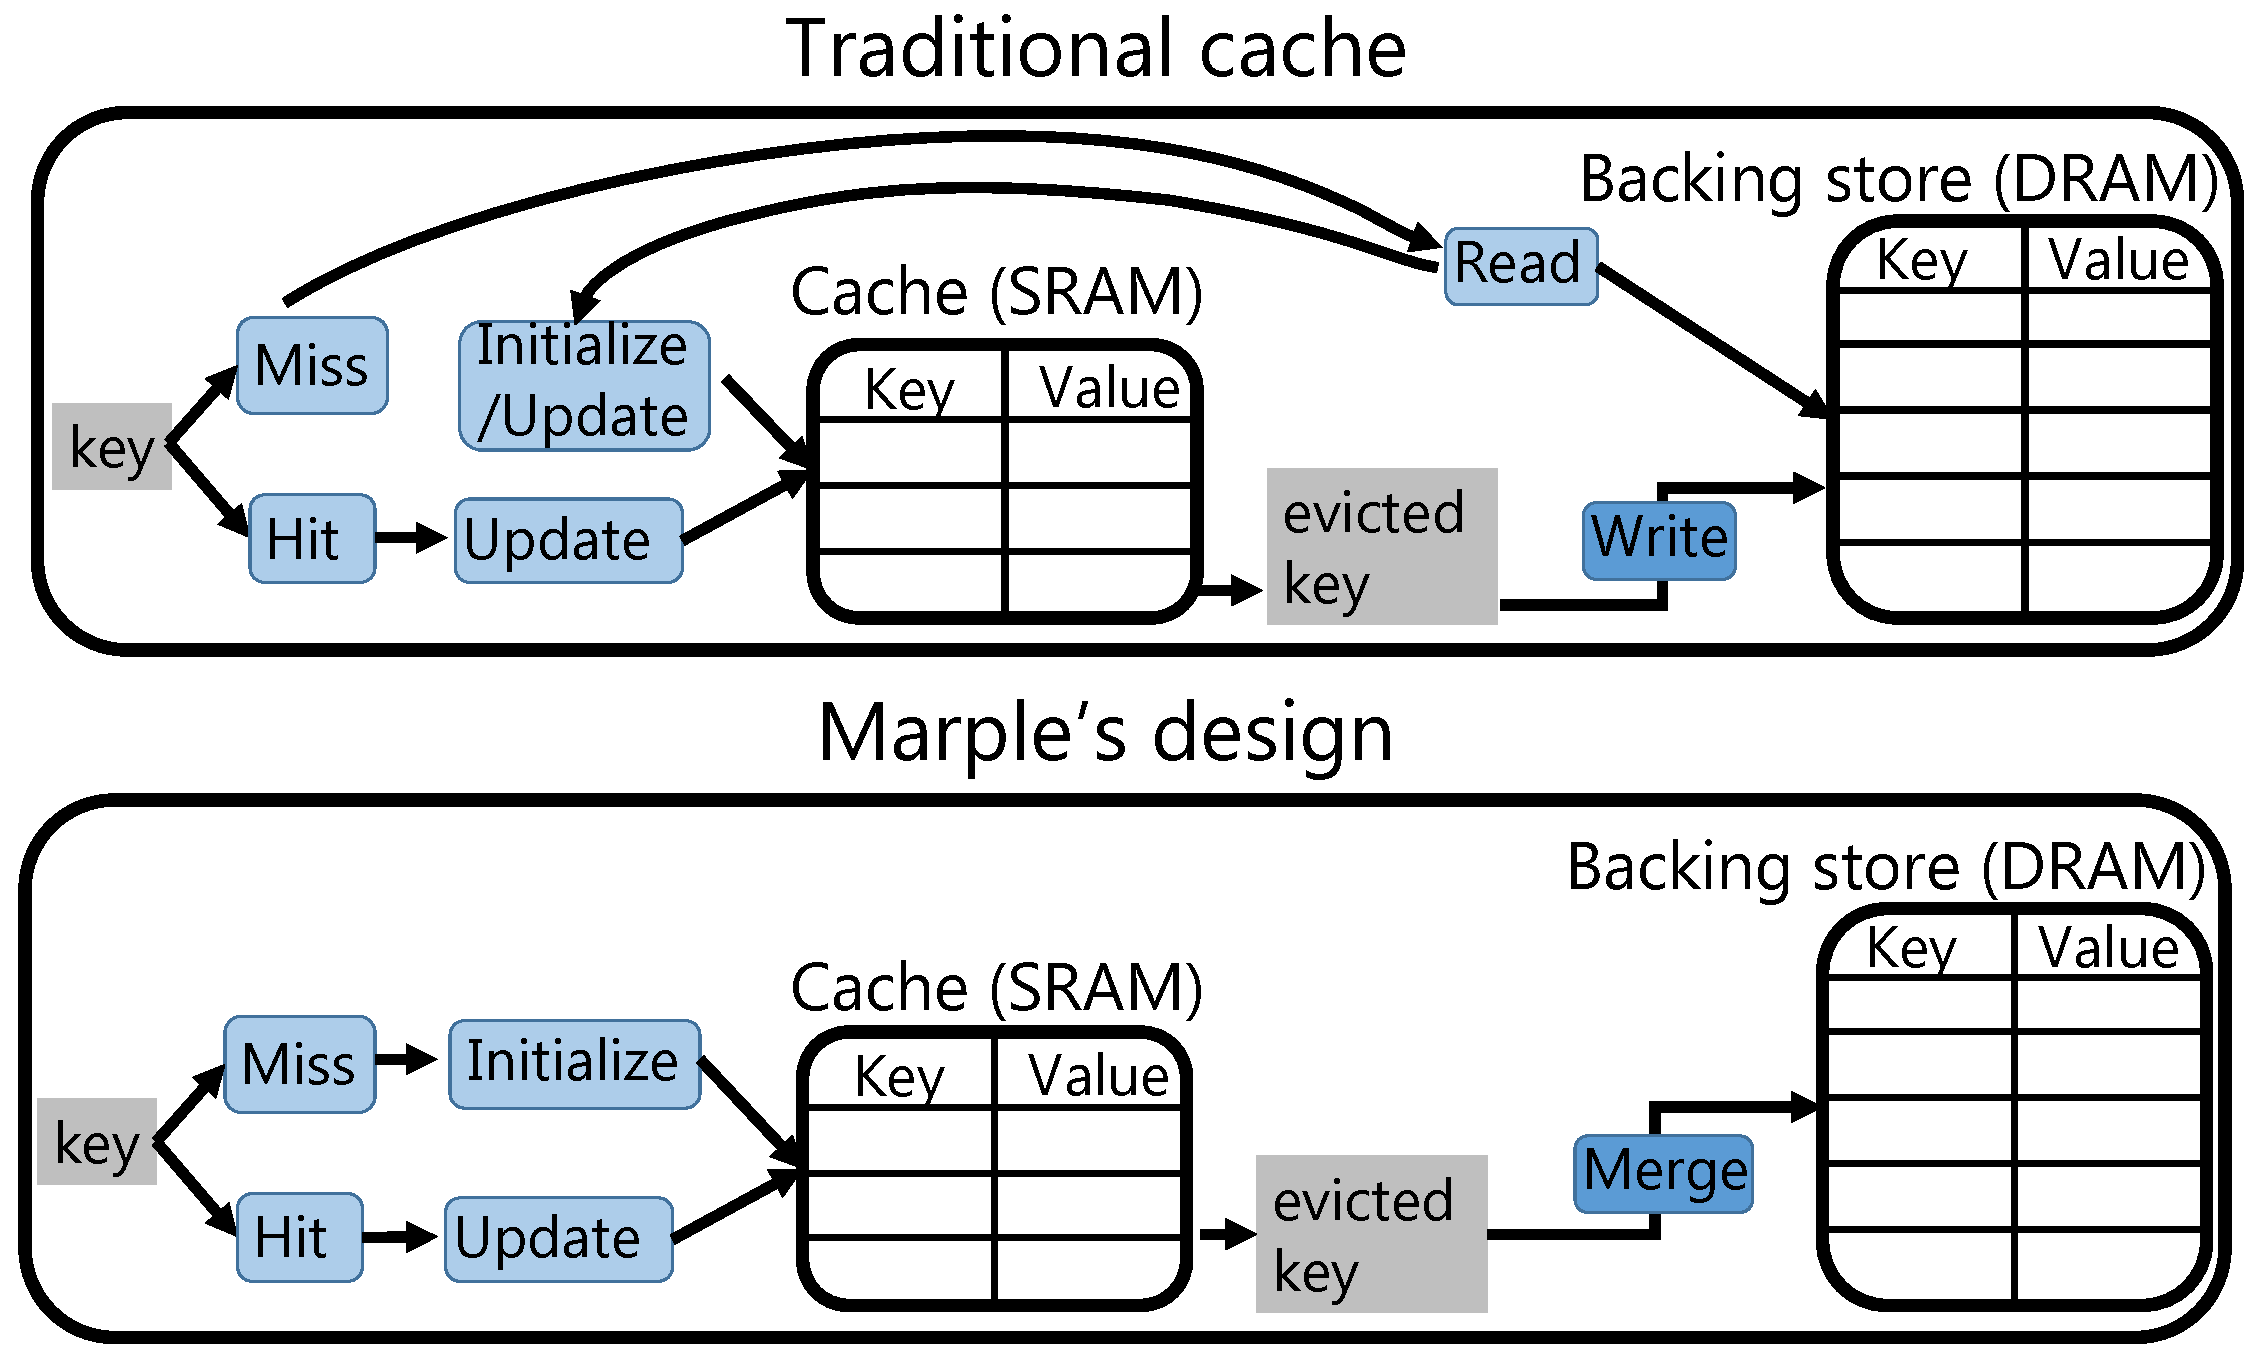
\includegraphics[width=\columnwidth]{pq_kv_store.pdf}
\caption{\TheSystem's key-value store vs. a traditional cache}
\label{fig:kv}
\end{figure}

We design our key-value store to process packets at line rate even on cache
misses (\Fig{kv}). Instead of stalling the pipeline waiting for a result from
DRAM, we treat the incoming packet as the first packet from a new flow and
initialize the flow's state to an initial value. Subsequent packets from the
same flow are aggregated within the newly created flow entry in the key-value
store, until the flow is evicted. When it is evicted, we merge the flow's value
just before eviction with its value in the backing-store using a {\em merge
function}, and write the merged result to the backing store. In our design, the
switch only writes to the backing store but never reads from it, which helps
avoid non-deterministic latencies.  The backing store may be
stale relative to the on-chip cache if there have been no recent evictions. We
remedy this by forcing periodic evictions.

To merge a flow's new aggregated value in the switch cache with its old value in the backing store
correctly, the cache needs to maintain and send {\em auxiliary state} to the
backing store.  A \naive usage of auxiliary state is to store relevant fields
from every packet of a flow, so that the backing store can simply run the
aggregation function over the entire packet stream when merging.  However, in a
practical implementation, the auxiliary state should be bounded in size and not
grow with the number of packets in the flow. Over the next four subsections, we
describe two classes of queries that are {\em mergeable} with a small amount of
auxiliary state (\S\ref{sec:associative} and
\S\ref{sec:linear-in-state-description}), discuss queries that are not
mergeable (\S\ref{sec:workaround-nonscalable}), and provide a general condition
for mergeability that unifies the two classes of mergeable queries and 
separates them from non-mergeable queries (\S\ref{sec:unifies}).
%TODO: Consider adding Amy's Venn diagram

\subsection{The associative condition}
\label{sec:associative}

A simple class of mergeable aggregations is associative functions.
Suppose the aggregation function on state $s$ is $s = op(s, f)$,
where $op$ is an associative operation and $f$ is a packet field. Then, if $op$
has an identity element $I$ and a flow's default value on insertion is $s_0 =
I$, it is easy to show that this function can be merged using the function
$op(s_{backing}, \scache)$, where $s_{backing}$ and $\scache$ are the value in
the backing store and the value just evicted from the cache, respectively. The
associative condition allows us to merge aggregation functions like addition,
max, min, set union, and set intersection.
% \MA{Consider defining identity element as a footnote}

\subsection{The linear-in-state condition}
\label{sec:linear-in-state-description}

Consider the EWMA aggregation function, which maintains a moving
average of queueing latencies across all packets within a flow. The aggregation
function updates the EWMA $s$ as follows:
\[ s = (1 - \alpha) \cdot s + \alpha \cdot (t_{out} - t_{in}) \]
We initialize $s$ to $s_0$. Suppose a flow $F$
is evicted from the on-chip cache for the first time and written to the backing
store with an EWMA of $s_{backing}$.\footnote{When a flow is first evicted, it does
not need to be merged.} The first packet from $F$ after $F$'s eviction is
processed like a packet from a new flow in the on-chip cache, starting with the
state $s_0$. Assume that $N$ packets from $F$ then hit the on-chip cache,
resulting in the EWMA going from $s_0$ to $\scache$.
Then, the correct EWMA $s_{correct}$ (\ie for all packets seen up to this point) satisfies:
\begin{align*}
s_{correct} - (1-\alpha)^N s_{backing} &= \scache - (1-\alpha)^N s_0 \\
s_{correct} &= \scache + (1-\alpha)^N(s_{backing} - s_0)
\end{align*}
So, the correct EWMA can be obtained by: (1) having the on-chip cache store
$(1-\alpha)^N$ as auxiliary state for each flow after each update, and
(2) adding $(1-\alpha)^N(s_{backing} - s_0)$ to $\scache$ when merging
$\scache$ with $s_{backing}$.

We can generalize this example. Let $\mathbf{p}$ be a
vector with the headers and performance metadata from the last $k$
packets of a flow, where $k$ is an integer determined at query
compile time (\S\ref{sec:linear-in-state-compilation}).
We can merge any aggregation function with state updates of the form
$\boldsymbol{S} = \boldsymbol{A}(\mathbf{p}) \cdot
\boldsymbol{S} + \boldsymbol{B}(\mathbf{p})$, where
$\boldsymbol{S}$ is the state, and
$\boldsymbol{A}(\mathbf{p})$ and $\boldsymbol{B}(\mathbf{p})$ are
functions of the last $k$ packets. We call this condition the
{\em linear-in-state} condition and say that $\boldsymbol{A}(\mathbf{p})$
and $\boldsymbol{B}(\mathbf{p})$ are functions of {\em
bounded packet history.}

The requirement of bounded packet history is important.
Consider the TCP non-monotonic query from \Fig{example-perf-queries}, which
counts the number of packets with sequence numbers smaller than the maximum
sequence number seen so far. The aggregation can be expressed as
\begin{lstlisting}
count = count + (maxseq > tcpseq) ? 1 : 0
\end{lstlisting}
While the update superficially resembles $\boldsymbol{A}(\mathbf{p}) \cdot \boldsymbol{S} +
\boldsymbol{B}(\mathbf{p})$, the coefficient $\boldsymbol{B}(\mathbf{p})$ is a function of {\ct
maxseq}, the maximum sequence number so far, which could be arbitrarily far
back in the stream.
%
Intuitively, since $\boldsymbol{B}(\mathbf{p})$ is not a function of bounded packet history,
the auxiliary state required to merge {\ct count} is large.
\Sec{unifies} formalizes this intuition.

In contrast, the slightly modified TCP out-of-sequence query from \Fig{example-perf-queries} {\em is}
linear-in-state because it can be written as
\begin{lstlisting}
count = count + (lastseq > tcpseq) ? 1 : 0
\end{lstlisting}
where {\ct lastseq}, the previous packet's sequence number, depends only on the last 2 packets: the current and the previous packet. Here,
$\boldsymbol{A}(\mathbf{p})$ and $\boldsymbol{B}(\mathbf{p})$ are functions of bounded packet history,
with $k = 2$.
%  This is in contrast to {\ct maxseq}, which depends on all packets seen so far.

Merging queries that are linear-in-state requires the switch to store
the first $k$ and most recent $k$ packets
for the key since it (re)appeared in the key-value store; details are
available in the appendix (Appendix~\ref{app:merge}).

An aggregation function is linear-in-state
if, for every variable in the function, the state update
satisfies the linear-in-state condition. A query is linear-in-state
if all its aggregation functions are linear-in-state.

\subsection{Scalable aggregation functions}
\label{sec:scalable}
A {\ct groupby} with no {\ct emit()} and a linear-in-state (or associative) aggregation function
can be implemented scalably without losing accuracy. Examples of such
aggregations (from \Fig{example-perf-queries}) include tracking successive
packets within a TCP connection that are out-of-sequence and counting the
number of TCP timeouts per connection.
%

 If a
{\ct groupby} uses an {\ct emit()} to pass tuples to another query, it cannot be
implemented scalably even if its aggregation function is linear-in-state or associative. An {\ct emit()} outputs the current state of the
aggregation function, which assumes the current state is always available in
the switch's on-chip cache. This is only possible if flows are never evicted,
effectively shrinking the key-value store to its on-chip cache alone.

\subsection{Handling non-scalable aggregations}
\label{sec:workaround-nonscalable}
While the linear-in-state and associative conditions capture several
aggregation functions and enable a scalable implementation, there are two
practical classes of queries that we cannot scale: (1) queries with aggregation
functions that are neither associative nor linear-in-state and (2) queries where
the groupby has an {\ct emit()} statement.

An example of the first class is the TCP non-monotonic query discussed earlier.
An example of the second class is the flowlet size histogram
query from~\Fig{example-perf-queries}, where the first {\ct groupby} emits
flowlet sizes, which are grouped into buckets by the second {\ct groupby}.

There are workarounds for non-scalable queries. One is to rewrite queries to
remove {\ct emit()}s.  For instance, we can rewrite the loss rate query
(\Fig{example-perf-queries}) to independently record the per-flow counts for
dropped packets and total number of packets in separate key-value stores, and
have an operator consult both key-value stores every time they need the loss
rate. Each key-value store can be scaled, but the implementation comes at a
transient loss of accuracy relative to precisely tracking the loss rate after
every packet using a {\ct zip.} Second, an operator may be content with flow
values that are accurate for each time period between two evictions, but not
across evictions (\Fig{accuracy-time}). Third, an operator may want to run a
query to collect data until the on-chip cache fills up and then stop data
collection.  Finally, if the number of keys is small enough to fit in the cache
(\eg if the key is an application type), the system can provide accurate
results without evicting any keys.

\subsection{A unified condition for mergeability}
\label{sec:unifies}
We present a general condition that separates mergeable functions from
non-mergeable ones.
Informally, mergeable aggregation functions are those that maintain auxiliary state
linear in the size
of the function's state itself.
This characterization also has the benefit of unifying the associative and
linear-in-state conditions.
We now formalize
our results in the form of several theorems without proofs; an accompanying
technical report~\cite{theory-tr} contains the proofs.

Let $n$ denote the size of state (in bits) tracked in a \TheSystem query: it must be
bounded and should not increase with the number of packets.  When merging state
$s_{cache}$ in the on-chip cache with state $s_{backing}$ in the backing store, the
switch may maintain and send auxiliary state $aux$  for the backing store to
perform the merge correctly.
In the EWMA example, the value
$(1-\alpha)^N$ is auxiliary state.
%%Note that the backing store may have its own
%%auxiliary state $a_{backing}$ to enable the merge.
Then, a \emph{merge function} $m$ for an
aggregation function $f$ is a function satisfying:
%%\[ m(s, aux, s_{backing}, a_{backing}) = f(s_0, \{p_1, \ldots, p_N\}) \]
\[ m(s_{cache}, aux, s_{backing}) = f(s_0, \{p_1, \ldots, p_N\}) \]
for any $N$ and sequence of packets $p_1, \ldots, p_N$. The application of $f$
to a list is shorthand for folding $f$ over each packet in order.

First, we show that \emph{every} aggregation function has a merge function,
provided it is allowed to use a large amount of auxiliary data.
%%\vspace{-0.18in}
\begin{theorem}
Every aggregation function has a corresponding merge function that uses
$O(n2^n)$ auxiliary bits.
\end{theorem}
\noindent
Unfortunately, memory is limited and \TheSystem should not use much more state
than indicated by the user's aggregation function.  We say an aggregation
function is \emph{mergeable} if the auxiliary state has size $O(n)$ for any
sequence of packets.  This characterization is consistent with what we
have described so far:
%
the linear-in-state and associative
conditions are indeed mergeable by this definition, while queries that we
cannot merge (\eg TCP non-monotonic in \Fig{example-perf-queries}) violate it.
\begin{theorem}
If an aggregation function is either linear-in-state or associative, it has a merge function
that uses $O(n)$ bits of auxiliary state.
\end{theorem}
\begin{theorem}
The TCP non-monotonic query from \Fig{example-perf-queries} requires $\Theta(n2^n)$ auxiliary bits
in the worst case.
\end{theorem}
\noindent
This raises the question: can we determine whether an aggregation function is
mergeable with $O(n)$ auxiliary bits? We provide an algorithm (described in the
tech report) that computes the minimum auxiliary state size needed to merge a
given aggregation function. Our current algorithm uses brute force and is
doubly exponential in $n$. However, a
polynomial time algorithm is unlikely. We demonstrate a hardness result by
considering a decision version of a simpler version of this problem where the
merge function $m$ is given as input: given an aggregation function $f$ and
merge function $m$, does $m$ successfully merge $f$ for all possible packet
inputs?
\begin{theorem}
Determining whether a merge function successfully merges an aggregation function
is co-NP-hard.
\end{theorem}

The practical implication of this result is that there is unlikely to be a
general and efficient procedure to check if an arbitrary aggregation function
can be merged using a small amount of auxiliary state. Thus, identifying
specific classes of functions (\eg linear-in-state and associative) and
checking if an aggregation function belongs to these classes is the best we can
hope to do.

\subsection{Hardware feasibility}
\label{sec:hardware-feasibility}
We optimize our stateful hardware design for linear-in-state queries and break
it down into five components.  Each component is well-known; our main
contribution is putting them together to implement stateful queries.
%One important design choice for a switch designer is how much memory to
%provision for the on-chip cache, which we evaluate in \Sec{eval}.
We now discuss each component in detail.

%Removed 128-bit key and 32-bit value because we evaluate different key and value sizes in eval
\textbf{The on-chip cache} is a hash table where each row in the hash table
stores keys and values for a certain number of flows. If a packet from a new
flow hashes into a row that is full, the least recently used flow within that
row is evicted. Each row has 8 flows and each flow stores both its key and
value.\footnote{The LRU policy is actually implemented across 3-bit pointers
that point to the keys and values in a separate memory. So we shuffle only the
3-bit pointers for the LRU, not the entire key and value.} Our choice of 8
flows is based on 8-way L1 caches, which are very common in
processors~\cite{intel_opt_manual}. This cache eviction policy is close to an
ideal but impractical policy that evicts the least recently used (LRU) flow
across the whole table (\Sec{eval}).

Within a switch pipeline stage, the on-chip cache has a logical interface
similar to an on-chip hash table used for counters:
each packet matches entries in the table using a key
extracted from the packet header, and the corresponding action (\ie increment)
is executed by the switch.
%
An on-chip hash table may be used as a path to incrementally deploying a switch
cache for specific aggregations (\eg increments), on the way to supporting
more general actions and cache eviction logic in the future.

\textbf{The off-chip backing store} is a scale-out key-value store such as
Redis~\cite{redis} running on dedicated collection servers within the network. As \Sec{eval}
shows, the number of measurement servers required to support typical eviction
rates from the switch's on-chip cache is small, even for a \hundredgswitch switch.

\textbf{Maintaining packet history.} Before a packet reaches the pipeline stage
with the on-chip cache, we use the preceding stages to precompute
$\boldsymbol{A}(\mathbf{p})$ and $\boldsymbol{B}(\mathbf{p})$ (the functions of bounded packet history)
in the state-update operation $\boldsymbol{S} =\boldsymbol{A}(\mathbf{p}) \cdot
\boldsymbol{S} + \boldsymbol{B}(\mathbf{p})$.
Our current design only handles the case
where $\boldsymbol{S}$, $\boldsymbol{A}(\mathbf{p})$, and $\boldsymbol{B}(\mathbf{p})$ are scalars. Say
$\boldsymbol{A}(\mathbf{p})$ and $\boldsymbol{B}(\mathbf{p})$ depend on packet fields from the last $k$
packets. Then, these preceding pipeline stages act like a shift register and
store fields from the last $k$ packets. Each stage contains a read/write
register, which is read by a packet arriving at that stage, carried
by the packet as a header, and written into the next stage's register. Once values from the last
$k$ packets have been read into packet fields, $\boldsymbol{A}(\mathbf{p})$ and
$\boldsymbol{B}(\mathbf{p})$ can be computed with stateless instructions provided by
programmable switch architectures~\cite{rmt, domino_sigcomm}.

\textbf{Carrying out the linear-in-state operation.} Once $\boldsymbol{A}(\mathbf{p})$ and
$\boldsymbol{B}(\mathbf{p})$ are known, we use a multiply-accumulate (MAC)
instruction~\cite{mac} to compute $\boldsymbol{A}(\mathbf{p}) \cdot \boldsymbol{S} +
\boldsymbol{B}(\mathbf{p})$. This instruction is very cheap to implement: our circuit
synthesis experiments show that a MAC instruction meets timing at 1 GHz and
occupies about 2000 \si{\micro\metre\squared} in a recent 32 nm transistor
library. A switching chip with an area of a few hundred
\si{\milli\meter\squared} can easily support a few hundred MAC instructions.

\textbf{Queries that are not linear-in-state.} We use the set of stateful
instructions developed in Domino~\cite{domino_sigcomm} for queries that are not
linear-in-state. Our evaluations show that these instructions are sufficient
for our example queries that are not linear-in-state.
